\chapter{稀土元素发展和新材料应用初探}

随着科学技术的发展,人类的社会形态和生活方式在近几个世纪不断被革新。尤其是二十世纪以来,各类基础学科的重大发现和扩展应用加速了这一变化。具体到化学而言,十九世纪出现的水泥和钢筋混凝土,伴随着石油提炼方式的创造,带领着人类走入材料和能源的新纪元。二十世纪初投入工业制造和研究的无机金属和有机材料两大方向,则更是与前者相辅相成。\cite{gan2014da}

稀土元素也在此时发现并被投入到一些生产应用上。步入六十年代 ,伴随着稀土矿场的大规模开采和钐钴永磁体的发明,稀土元素开始了它的表演——它陆续被应用在电气原件生产和反应催化处理中,并在新世纪被赋能为新能源器械的灵魂元素。正因如此,在稀土元素的开采、加工、利用各阶段,我们要更好地运用绿色化学的思想,助力可持续发展,为碳中和贡献自己的力量。\cite{Atwood_2012,Balaram_2019,Institute_2020}

本文将基于上述背景,从化学和智能生活的角度出发,探究稀土元素在新材料中的应用。

\section{分类及开采}

\begin{figure}[H]
    \centering
    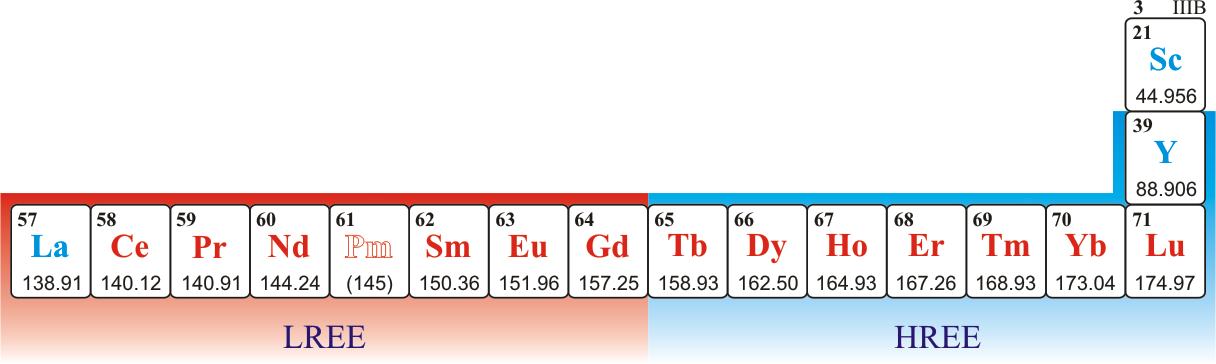
\includegraphics[width=0.9\columnwidth]{../images/ree_division.png}
    \caption{展示了稀土元素在元素周期表的位置和一种分类。\cite{Generalic_2012}\label{fg:division}}
\end{figure}
稀土元素(REE, Rare Earth Element),指的是元素周期表上第IIIB族的17种元素,包括钪(Scandium)、钇(Yttrium)和含镧(Lanthanum)在内的其他十五个镧系元素,并共享着类似的化学性质,例如:在简单化合物中,由于各元素原子的电子分布情况类似(\ce{4f^{0$\sim$14} 5d^{0$\sim$1} 6s^{2} }),最后增加的电子一般填充在f亚层中,它们均以正三价的形式存在。与之相对应的,粒子微小的变动导致它们之间有所区别,例如:钷(Promethium)是这些元素里的唯一一个放射性元素(严格来说也不算化学性质了)。另外,根据矿物分布及特征,和粒子半径及其导致的不同性质,稀土元素还被分为轻型重型两类,一种常见区分方法及其在元素周期表内的位置如\autoref{fg:division}。不同的分类方法\cite{Generalic_2012,Atwood_2012,baipi_2012}可能会从钐(Samarium)到镝(Dysprosium)选择某个元素作为重稀土(HREE, Hard Rare Earth Element)起始元素,而钪则一般不像钇一样归入重稀土元素,也不归入轻稀土(LREE, Light Rare Earth Element),而是单独成一类。

\begin{figure}[H]
    \centering
    \includesvg[width=0.6\columnwidth, pretex=\tiny]{../images/elemental-abundances.svg}
    \caption{展示了部分元素的各类型粒子在地球土壤中的丰度。\cite{Haxel_2002}\label{fg:abundances}}
\end{figure}

值得一提的是,稀土的名称正来源于“稀有的土壤成分”,但现代的地质学考证结果说明,它们的含量远比我们熟知的珍贵金属(Precious metals),如银、金等要高一个数量级。而铈(Cerium)作为地球土壤中丰度最高的稀土元素,更是得到了第27名的好成绩。可视化的数据可以看\autoref{fg:abundances},这张广泛引用的相对丰度图有力地展现了稀土元素的高含量。相比较而言,陨石中稀土元素含量往往还更少。\cite{Balaram_2019}

和老朋友铝很像,稀土元素的发现和制备的相关历史均较短,这和稀土元素活泼的性质是分不开的——他们在土壤矿质中均以化合物的形式存在,且各种元素混合在一起,需要合适的工艺进行分离,低效的工艺可能会将大量有效成分作为难以分离的杂质丢弃。\cite{Atwood_2012,张晔_2019}由于篇幅所限,此处不过多涉及开采和矿类加工的相关内容,这些信息在中文互联网上满地都是。(不会吧,不会真有人不知道中国的稀土勘探量和产量名列前茅吧)

\section{工业应用情况}

稀土早期曾应用于燃气灯覆盖层、抛光物质和玻璃上色等工艺中,而要系统地介绍当前稀土元素的各类用途和场景是很困难的。基于写一篇小论文的目标,此处不区分各元素地描述和日常场景相接近的三个用途:催化、磁性和超导,将简单介绍其相应的化学原理和实际应用产品。

稀土还用于荧光粉、玻璃添加剂、合金和有机材料合成等相关领域\cite{JohnHamiltonWalrod_2012a,Dawei_2018,DeakinUniversity_2012},但需要前置知识过多,而且内容杂碎,故这些应用虽然也很重要但此处不再涉及。

\subsection{用于催化过程}

稀土元素最早的工业应用,便是作为多相催化物(Heterogeneous Catalysis)用于冶金和石油化工工业。

在冶金工业中它们作为还原剂、脱氧剂和脱硫剂。在炼钢温度下反应\ce{2La + 3[O] <=>[1600 \textdegree{C}C] La2O3(s) }可很快发生平衡,例如钢中只要含$2\times10^{-4}\%$的镧,它的含氧质量分数便可降低至$1\times10^{-4}\%$。\cite{gan2014inbook}

同时,液化的稀土氧化物可取代传统的强酸强碱,在化工反应中替代沸石晶格中的某些重要成分,产生大量能量,并导致石油等物质催化裂化,甚至于酯的水解。值得注意的是,它们在600~800K以上的温度才有催化活性。\cite{JohnHamiltonWalrod_2012,金文_2015}
据记载,典型的催化氧化物有氧化铈(\ce{CeO2})、氧化镧(\ce{La2O3})和氧化钕(\ce{Nd2O3}),它们作为催化剂在2008年的年度消耗量就分别达到了6840 mt,380 mt和228 mt。\cite{Atwood_2012a}

作为多相催化物,稀土元素还有可能在汽车尾气处理、锅炉烟尘等方向继续发挥作用,促进尾气处理,实现环保的目标。如南京大学董林教授就在进行低温稀土铈基催化剂脱硝的研究和实践。\cite{张晔_2019}\footnote{\inlinecite{张晔_2019}这篇采访稿里其实有很多值得推敲的地方,比如\inlinecite{Atwood_2012a}就提到国际上销量最多的稀土元素应该是Ce, La, Nd, 全是轻稀土}此外,稀土作为均相催化剂(Homogeneous Catalysis)与有机物等物质相结合,也是目前研究的热点方向。\cite{Yao_2012a}

\subsection{用于磁性材料}

正如前述所言,稀土金属最早展现出了它在磁体方面的魅力,直到现在新材料、新科技的应用时代,这点仍显得尤为重要。就连加拿大某矿产公司主营市场经销的Pierre Neatby也坦言:“像钕磁铁,能做到重量轻而又有强磁力,所以用它来作电动汽车的引擎,就能更好地让它轻量化、小型化。正因如此,从\textbf{喷气飞机到军用潜艇再到新能源汽车},稀土元素都发挥着独特的作用。”\cite{Kirkpatrick_2019}就具体数据而言,一个3.5兆瓦功率的涡轮\textbf{风力发动机},便需要600千克的稀土永磁体材料。\cite{Atwood_2012a}

由于居里温度低,在室温下纯稀土物质并不显现磁性,但与过渡金属铁镍等形成化合物后,其磁性比铁氧体磁铁或陶瓷磁铁均要更强。它们的磁性来源于原子结构造成的高磁矩(4f轨道上未成对电子同向自旋),以及晶体结构的高磁向各异性。

传统来说,钕铁硼磁铁和钐钴磁铁(当然还含其他物质)这两种是最常见的永磁体。而未来对稀土磁体的研究,可能可以从不同的磁体排序材料,如链状磁、离子磁、原子磁等(SCM = single-chain magnets; SIM = single-ion
magnet; SMM = single-molecule magnets)\cite{Wang_2012a,Wang_2012}

\subsection{用于超导材料}

超导材料指的是在特定温度和压强下展现出零电阻的物质,且环境一般是低温高压(毕竟超导也是追求绝对零度的科研副产品)。所谓的\qthis{高温超导材料}(HTSC, high temperature superconductors)反而是指77K以上(液态氮气环境)可展现超导性质的物质,在这个条件下的超导将具有更为普遍的实用意义。

稀土元素很早就被用来进行高温超导研究,并在本世纪初利用稀土实现了120K以上的超导物质(见\autoref{fig:sc2012}),在去年更是有学者实现了室温高压的超导(居然不带稀土玩了,虽然你看发展轴上全是稀土,见\autoref{fig:sc2020})。

\begin{figure}[H]
	\begin{minipage}{0.45\textwidth}
		\centering
		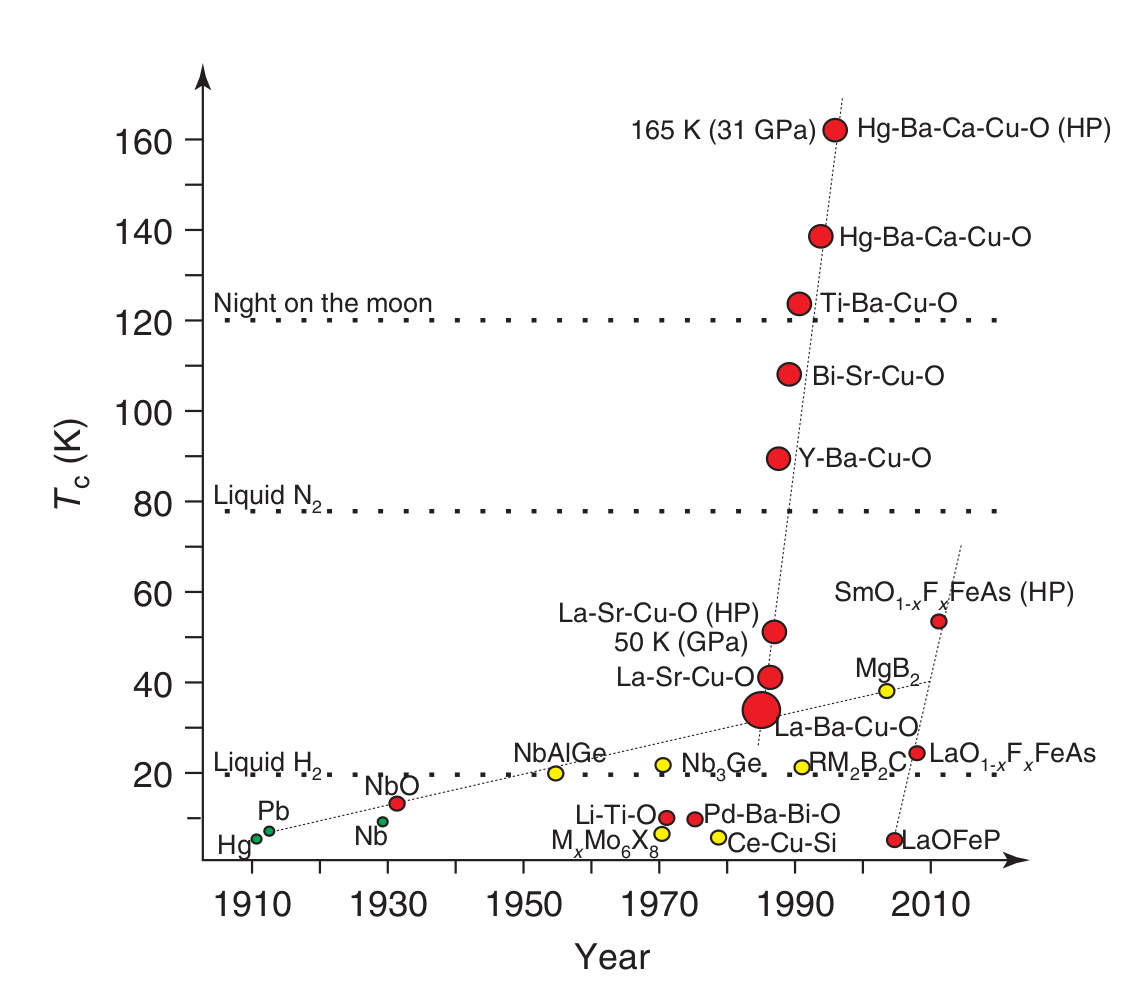
\includegraphics[width=1.05\columnwidth]{../images/superconduct1.png}
		\caption{\inlinecite{AntonioJ.DossantosGarcia_2012a}中展示的超导进化树}
		\label{fig:sc2012}
	\end{minipage}\hfill
	\begin{minipage}{0.45\textwidth}
		\centering
		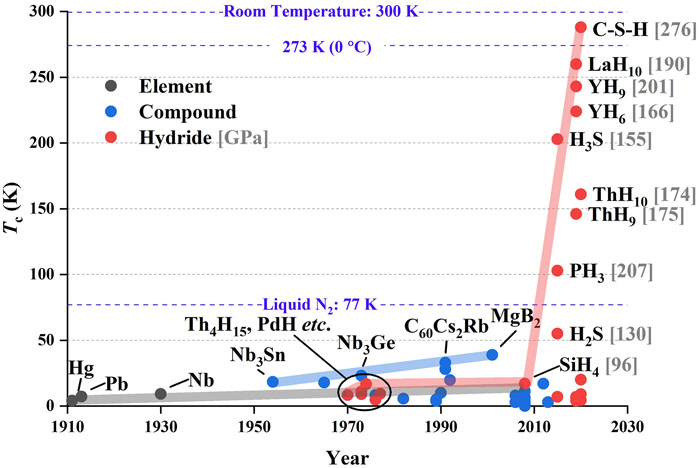
\includegraphics[width=1.05\columnwidth]{../images/superconduct2.jpg}
		\caption{\inlinecite{Lv_2020}中展示的超导进化树}
		\label{fig:sc2020}
	\end{minipage}
\end{figure}

距离我们生活最近的超导材料便是磁悬浮(它和强磁性无关),它应用了迈斯纳效应(Meissner effect),西南交通大学的超高速真空管道磁悬浮交通研究中心正力图从传统的电磁悬浮、电动悬浮两种磁悬浮方式中吸收经验,利用研究成果应用于高温超导悬浮。2021年1月,设计时速620公里的样车和设计线已与媒体见面,其技术和制造工艺均为国产原创,它是西南交通大学联合中车公司、中国中铁等单位协同攻关研发的项目,旨在让技术走出实验室,迈出验证其高速运行可靠性的第一步。高温超导甚至还可以用于普通马达的储能,这也将是一个前沿应用方向\cite{AntonioJ.DossantosGarcia_2012a,王迪_2021}

题外话:如果用超导微观的BCS理论(Bardeen–Cooper–Schrieffer theory)来研究这个现象,那么这些稀土元素的磁性和超导特性的原理都是一样的。另外如果只涉及到导体,钕和钐的氧化物还是陶瓷电容(C0G (NP0))的主要成分,这种电容具有温度补偿特性,是电容量及介质损耗最稳定的电容器之一。具体来说,集成电路上广泛用到这种电容。\cite{Kaye_2020}

\section{结语}

本文通过简述传统化工材料的路径,并描绘稀土元素和新材料的发展,展现了当下化学知识及其应用与智能生活密不可分的关系,运用这些知识有助于我们构造环境友好型社会。同时,\inlinecite{Atwood_2012}这本书对稀土的基本化学性质、有代表性的化合物、以及一些常见形态和应用方式进行了说明,对我撰写上述内容时起到了很大的帮助(同时有些专业知识也让我陷进去了)。根据系列序言,该书是EIBC(Encyclopedia of Inorganic and Bioinorganic Chemistry)的一部分,并旨在为初学者和研究者提供翔实的参考资料。

需要注意本文引用的数据仅供说明使用,不构成任何对比或事实阐述,含数字的内容均有文献参考,但其准确性仅供参考。市场分析自己去看,不构成投资建议。\cite{baipi_2012,Fernandez_2017}(说白了,定性说话不腰疼,定量说话要挨打)

参考文献等原始数据,参见\url{https://github.com/tiger3018/hw/blob/HEAD/chemistry}。